\documentclass[11pt, oneside]{article}   	% use "amsart" instead of "article" for AMSLaTeX format
\usepackage{geometry}                		% See geometry.pdf to learn the layout options. There are lots.
\geometry{letterpaper}                   		% ... or a4paper or a5paper or ... 
%\geometry{landscape}                		% Activate for rotated page geometry
%\usepackage[parfill]{parskip}    		% Activate to begin paragraphs with an empty line rather than an indent
\usepackage{graphicx}				% Use pdf, png, jpg, or eps§ with pdflatex; use eps in DVI mode
								% TeX will automatically convert eps --> pdf in pdflatex		
\usepackage{amssymb}
\usepackage{amsmath}
\usepackage{hyperref}

%SetFonts
\usepackage[T1]{fontenc}
\usepackage{lmodern}



%----macros begin-----------------------------------------------------------------------------------
\usepackage{graphicx}
\usepackage{color}

\def\conv{\mbox{\textrm{conv}\,}}
\def\aff{\mbox{\textrm{aff}\,}}
\def\B{\mathbb{B}}
\def\N{\mathbb{N}}
\def\E{\mathbb{E}}
\def\R{\mathbb{R}}
\def\Z{\mathbb{Z}}
\def\v#1{{\bf #1}}
\def\p#1{{\bf #1}}
\def\T#1{{\bf #1}}
\def\vet#1{{\left(\begin{array}{ccccccc}#1\end{array}\right)}}
\def\mat#1{{\left(\begin{array}{ccccccc}#1\end{array}\right)}}

\def\lin{\mbox{\rm lin}\,}
\def\aff{\mbox{\rm aff}\,}
\def\pos{\mbox{\rm pos}\,}
\def\cone{\mbox{\rm cone}\,}
\def\conv{\mbox{\rm conv}\,}

\newcommand{\floor}[1]{\left\lfloor #1 \right\rfloor}
\newcommand{\ceil}[1]{\left\lceil #1 \right\rceil}
%----macros end-----------------------------------------------------------------------------------


% rules for for inputed tables
% the
\usepackage{siunitx}
\usepackage{booktabs}

%alternative rules for tables
%\newcommand{\toprule}{\hline}
%\newcommand{\midrule}{\hline}
%\newcommand{\bottomrule}{\hline}
%\newcommand{\specialrule}{}

%SetFonts


\title{Fast algebraic filtering of surfaces from 3D medical images with Julia}
\author{Miroslav Ji\v{r}\'ik and Alberto Paoluzzi}
\date{}							% Activate to display a given date or no date

\begin{document}
\maketitle

\begin{abstract}
In this paper we introduce a novel algebraic \textsc{lar-surf} filter, well founded on algebraic topology methods, to extract and smooth the boundary surface of any subset of voxels arising from the segmentation of a 3D medical image. The input is defined as a \emph{chain}, i.e.~as a vector from a linear space of 3-chains, represented in coordinates as a sparse Boolean vector. The output is produced as the result of the mapping via the linear boundary operator $\partial_3:C_3 \to C_2$ between linear spaces of 3- and 2-chains.  In particular, when the input set of voxels is either not (4-)connected, or contains one or more empty regions inside, \textsc{lar-surf} generates a non connected set of closed surfaces, i.e.~a set of 2-cycles---using the language of algebraic topology. The only data structures used by this approach are sparse arrays with one or two indices, i.e.~sparse vectors and matrices. This work is based on LAR (Linear Algebraic Representation) methods, and is implemented in Julia language, natively supporting parallel computing on hybrid architectures.
\end{abstract}

\tableofcontents

%\section{}
%\subsection{}

\section{Introduction}\label{sec:intro}


Isosurface extraction to produce geometric models of surfaces from volumetric data is important in many applications. It is often used for indirect visualization of the medical data or for flow modeling \cite{Rohan2018a}. 
% In this paper we suggest an approach based on 
 
% Input volumetric data are represented by a 3D voxel field and can be generated by segmentation of sections from computed tomography. 
The most popular algorithm used for surface extraction is probably Marching Cubes (MC). The algorithm was described by Lorentsen and Cline \cite{Lorensen1987} in 1987. The survey of Marching Cubes algorithms has been published in 2006 \cite{Newman2006}. The algorithm is based on considering the cube defining volume. Each corner vertex of the cube is related to input volumetric data. MC traverse the data and constructs the surface by using a lookup table of different triangular faces depending on different patterns of the cube.  The main disadvantages of this method are time requirements, ambiguity, and holes generation. Some of them were discovered shortly after the algorithm was introduced. 
Marching Cubes. In 1991 Nielson and Hamman described an Asymptotic Decider to solve the ambiguity problem on the faces of the cube.  Natarajan noted that the ambiguity problem also occurs with uniform samples \cite{Natarajan1994}. In 1995 Chernyaev extended the number of cases to 33 \cite{chernyaev1995marching}. More recently the algorithm was updated by Custodio, Pesco, and Silva to enhance the quality of iso-surface triangulation \cite{Custodio2019}. 

Some alternative methods have been developed, including a method for surface extraction using particle attraction; a system was described by Crossno and Angel in \cite{Crossno1997}. A graph processing that tracks the boundary cell-face adjacencies is described in \cite{Lachaud2000}. Some parallel algorithms for iso-surface extraction are discussed in \cite{Bajaj2004}.
A completely data-parallel algorithm, implemented in OpenCL that runs entirely on the GPU is presented in~\cite{Smistad12}. 
A Linear Algebraic Representation approach, parallelized using the OpenCL framework on Linux, was discussed in~\cite{Paoluzzi2016}. % \cite{paodcvjcadanda2015}.

% In this paper
% TODO slightly change the formulation
Here we discuss an alternative approach for surface extraction. Our \textsc{lar-surf} (Linear Algebraic Representation Surface extraction) filter is based on basic algebraic topology and linear algebra, using linear spaces $C_p$ of chains (of cells) of dimension $0 \leq p \leq 3$ and the boundary matrix $[\partial_3] : C_3 \to C_2$.

Input volumetric data are represented by a 3D voxel array and can be generated by segmentation computed tomography (upper left image on Fig. \ref{fig:example_liver_macro_micro}). A decomposition of the input volumetric data into small submatrices called \emph{bricks} is performed, then the binary coordinate vector of each interesting chain of voxels is generated, and its boundary is computed by matrix multiplication times the boundary matrix producing the binary representation of the boundary surface (the surface which defines the boundary). 
Embarrassing parallel data decomposition is used to compute the boundary surface patches within each of the bricks, that are finally joined and smoothed via the Taubin algorithm \cite{Taubin1995}.

The present paper is organized as follows.
Section~\ref{sec:background} provides the basic topological and geometrical concepts needed to understand the \textsc{lar-surf} method, including the building of boundary matrices, the map from Cartesian indices to linear indices, and the Taubin smoothing method.
Section~\ref{sec:filter} discusses the parametric design of the unit block filtered by the parallel algorithm, including the block decomposition, the sparsity rate of the used sparse arrays, and the block-level parallelism.
Section~\ref{sec:julia} is related to the algorithm implementation in Julia, and in particular to a discussion of the parallel workflow.
Section~\ref{sec:examples} presents some examples of algorithm execution on the liver and the hepatic portal system.
Section~\ref{sec:conclusion} shortly describes the next extensions of this approach, in particular the implementation with Julia's support for GPU parallelism and the multi-segmentation of Medical images.


\section{Background}\label{sec:background}

Some basic concepts of solid modeling, and in particular the foundational idea of representation scheme, as well as few basic concepts of algebraic topology, are shortly introduced in this section, including the computation of the matrix of a boundary operator between chain spaces.

\subsection{Representation Scheme}\label{sec:schemes}

A \emph{representation scheme} for solid modeling is a mapping between a space of mathematical models and  space of symbolic representations like generated by a formal grammar.
Solid pointsets (i.e., `$r$-sets') are defined~\cite{Requicha:1980:RRS:356827.356833} as compact (bounded and closed) regular and semianalytic subsets of the $d$-space. A large number of representation schemes were defined in the past forty years, including the two main classes of (a) \emph{boundary representations} (`$B$-reps'), where the solid model is represented through a representation of its boundary elements, i.e.~faces, edges and vertices, and (b) \emph{decompositive/enumerative representations} \cite{Requicha:1980:RRS:356827.356833}, that are a decomposition of either the object or the embedding space, respectively, into a well-defined \emph{cellular complex}. In particular, a boundary representation provides a cellular decomposition of the object's boundary into \emph{cells} of dimension zero (vertices), one (edges), and two (faces). Medical imaging can be classified as the \emph{enumerative representation} of cellular decompositions of organs and tissues of interest \cite{Paoluzzi2016}, in particular, as subsets \emph{of 3D volume elements} (voxels) from the 3D image. 


\subsection{Linear Algebraic Representation}\label{sec:lar}


The \emph{Linear Algebraic Representation} (\textsc{lar}), introduced in~\cite{Dicarlo:2014:TNL:2543138.2543294}, aims to represent the \emph{chain complex}~\cite{TSAS,DiCarlo2009} generated by a piecewise-linear \emph{geometric complex} embedded either in 2D or in 3D. In a few words, it gets a minimal characterization of geometry and topology of a cellular complex, i.e.~the embedding mapping $\mu : C_0 \to \E^d$ of 0-cells (vertices), as well a description of $(d-1)$-cells as subsets of vertices, and is able to return the whole chain complex 
\begin{equation}
C_\bullet = (C_p, \partial_p) := 
C_3 
\substack{
\delta_2 \\
\longleftarrow \\
\longrightarrow \\
\partial_3 
}
C_2 
\substack{
\delta_1 \\
\longleftarrow \\
\longrightarrow \\
\partial_2 
}
C_1  
\substack{
\delta_0 \\
\longleftarrow  \\
\longrightarrow \\
\partial_1 
}
C_0 .
\end{equation}



%\[ 
%C_\bullet = (C_p, \partial_p) := 
%C_3 \ 
%\substack{
%\delta_2 \x
%\longleftarrow \[-1mm]
%\longrightarrow \
%\partial_3 
%}
%\ C_2 \ 
%\substack{
%\delta_1 \
%\longleftarrow \[-1mm]
%\longrightarrow \
%\partial_2 
%}
%\ C_1 \ 
%\substack{
%\delta_0 \
%\longleftarrow \[-1mm]
%\longrightarrow \
%\partial_1 
%}
%\ C_0 .
%\] 

% {   
%   \centering\vspace{1mm}
%   \includegraphics[width=0.475\textwidth]{figs/complex} 

% }

\noindent
and, in particular, any basis for linear chain spaces $C_p$, and any linear
boundary/coboundary map \(\partial_p\) and
\(\delta_p=\partial_{p-1}^\top\) between them. The \emph{domain} of \textsc{lar} is the set of \textbf{chain complexes} generated by cell $d$-complexes ($2\leq d\leq 3$). The computer \emph{representations} of \textsc{lar} are \textbf{sparse binary matrices} to represent both the operators and the chain bases. Note that in algebraic topology a $p$-chain is defined as a linear combination of $p$-cells with scalars from a field. When the scalar coefficients are from $\{-1, 0, +1\}$, a chain may represent \emph{any (oriented) subset of cells} from the cellular complex.
Scalars from $\{0, 1\}$ are used for non-oriented complexes.

We may, therefore, get the $(p-1)$-boundary $\partial_p c_p$ of \emph{any} $p$-chain $c_p$, by multiplication of the coordinate representation $[\partial_p]$ of the boundary operator times the coordinate representation $[c_p]$ of the chain in terms of such scalars, i.e.~by a  matrix-vector product $ [\partial_p] [c_p] $.

It is possible to show that the \textsc{lar} representation scheme is very expressive, i.e.~that it  has a large domain,  including collections of: line segments, quads, triangles, polygons, meshes;  pixels, voxels, volume images; B-reps, enumerative and decompositive representations of solids. 
In this paper we apply \textsc{lar} methods to computation of boundary representations of solid models from segmentation (labeling) of 3D medical images.
To display a triangulation of  boundary faces  in their proper position in space, the information required is contained in the \emph{geometric chain complex} (GCC):
\[
\mu: C_0\to\E^3,\ (\delta_0, \delta_1, \delta_2)
\qquad\equiv\qquad
\texttt{(geom, top) = (V, (EV, FE, CF))}
\]
The GCC allows to transform the (possibly non connected) boundary 2-cycle of surfaces as a standard B-rep~\cite{shapiroSM:202}. 
The geometry \texttt{geom} is given by
the embedding matrix \texttt{V} of vertices (0-cells), and  topology \texttt{top} by the three sparse matrices (\texttt{EV}, \texttt{FE}, \texttt{CF}) of coboundaries ($\delta_0, \delta_1, \delta_2$) of the chain complex describing a   
space arrangement~\cite{paoluzzi2019finite}.
Note that ordered pairs of letters from \texttt{V,E,F,C}, correspond to \emph{\emph{\texttt{V}}ertices$\to$\emph{\texttt{E}}dges$\to$\emph{\texttt{F}}aces$\to$\emph{\texttt{C}}ells} into the 
\emph{\emph{\texttt{C}}olumn$\to$\emph{\texttt{R}}ow} order of matrix maps of operators.



\subsubsection*{Construction of boundary matrix $\partial_d$}

First, let us fix an ordering for all the cells of a partition of input data (with vertices $V$, edges $E$, pixels $F$, and voxels $C$), i.e.~for each 0-, 1-, 2-, and 3-elements of a cell partition \texttt{V,E,F,C} of a 3D image, i.e., once fixed the $p$-bases for linear spaces $C_p$ of $p$-chains $(0\leq p\leq 3)$, we call $M_p = (m_{i,j})$ the \emph{characteristic matrix} of the $p$-basis, expressed as subsets so that 
$m_{i,j}=1$ if and only if the $j$-th  $0$-cell $c^j_0$ belongs 
% , where  we have that $m_{i,j}=1$ if and only if the $j$-th $0$-cell belongs 
to the boundary of $i$-th $p$-cell $m_{i,j}$, and $m_{i,j}=0$ otherwise.  

Let us note that the product of binary matrices is not binary, so by computing the (sparse) matrix product $(M_{p-1} M_{p}^t) = (n_{i,j})$, with $n_{i,j} = \sum_{k} m_{i,k}m_{k,j}$, we get for each $n_{ij}$ the \emph{number of vertices} shared by $c_{p-1}^i$ and $c_{p}^j$. When this number equates the cardinality of $c_{p-1}^i$, this elementary chain is contained on the boundary of $c_{p}^j$. In a volumetric data, with cubic 3-cells and squared 2-cells in-between, everywhere we get $n_{i,j}=4$, we may state $c_{2}^i\subset\partial c_{3}^j$. Therefore, in each $j$ column of $M_{2} M_{3}^t = (n_{i,j})$, we have exactly \emph{six rows} where  $n_{i,j} = 4$, since a cube (3-chain) has six boundary faces (2-chains). The unit incidence coefficients in $\left[\partial_3\right]$ are accordingly located by filtering the coefficients with value 4.

Finally, consider the linear graded boundary operator $\partial_p : C_p \to C_{p-1}$. As such, it contains by columns the representation of domain basis elements, expressed as a linear combination of the basis elements of the range space. Therefore, the operator matrix $[\partial_d]$ is readily obtained by setting $[\partial_d](i,j)=1$ if $n_{i,j}=4$ and $[\partial_d](i,j)=0$ otherwise.  Of course, it will contain six non-zero elements for the column.  It may be worth remembering every 3-cell (voxel) of the volumetric data has exactly six 2-faces. 

It is possible to show that all the interesting relations of incidence/adjacency between cells of different dimensions can be both computed and efficiently queried by pairwise computing some matrix products, with one of terms possibly transposed, using only the two boundary and coboundary operator matrices $[\partial_p]$ and $[\delta_p]$, and where $[\delta_p] = [\partial_p^\top]$. We~may also show that such matrices are \emph{very sparse}, with their sparseness growing rapidly with the dimensions (see Section~\ref{sec:brick}). The pattern of non-zeros in matrix $[\partial_3]$ corresponding to a brick of shape $(4,4,4)$ is given in Fig.~\ref{fig:boundary_matrix_4x4x4}.

\begin{figure}[tbp] %  figure placement: here, top, bottom, or page
   \centering
   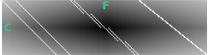
\includegraphics[width=0.75\linewidth]{src/figs/boundary_matrix_4x4x4_desc.png} 
   \caption{
   The binary image of \emph{sparse} coboundary matrix  $\left[\delta_2\right] = \left[\partial_3\right]^t : C_2 \to C_3$,
%   The binary image of the coboundary operator  $\delta_2 = \partial_3^\top : C_2 \to C_3$, 
   built for a small volumetric data (or a brick) with shape $(4,4,4)$. Note that the number of rows equates the size $4\times 4\times 4 = 64$ of the voxel set; the number of columns is $d\,n\,(1+n)^{d-1} = 3\times 4\times 25 = 300$. Of course, the number of non-zeros per row (cardinality of the facet set of a single voxel) is six, whereas the number of non-zeros per column is two, but on boundary facets.}
   \label{fig:boundary_matrix_4x4x4}
\end{figure}

\subsection{Multiindices from Cartesian indices}\label{sec:inds-from-cart}

In order to utilize the topological algebra shortly recalled in this paper, we need to explicitly sort the cells of the various dimensions into linearly ordered sequences, possibly according to the linear order their information is linearly accommodated in computer storage. 

\subsection{Taubin Smoothing}\label{sec:taubin}

Every boundary chain extracted from an image block $\B(i,j,k,n)$ is a \emph{2-cycle}, i.e., a closed 2-chain---in other words, a 2-chain with empty boundary. Such 2-cycles are joined together by removing the double 2-cells (at the boundaries of adjacent bricks) after having suitably shifted their indices to an unique linear representation of the whole image. The resulting raster surface is made by mutually orthogonal raster facets, that must be smoothed in order to get a fair surface. A linear time and space algorithm for this purpose is the Laplacian smoothing, which iteratively  moves each vertex (0-cell) to the centroid of its neighbors. A well known weakness of this simple algorithm is the asymptotic convergence of the whole mesh to a single point, resulting in unfair size reduction even after few iterations.  Conversely, the Taubin smoothing algorithm~\cite{Taubin:1995:SPA:218380.218473,egst.20001029} alternates two Laplacian smoothing steps with \emph{shrink} and \emph{inflate} effects respectively, with the result of delivering pretty invariant sizes and volume of the smoothed mesh. The best results are obtained on meshes which have small variations of edge length and face angles, like for surfaces extracted from 3D raster images, as in our case.
 



\section{Block-parametric design}\label{sec:filter}

\subsection{Block decomposition}\label{sec:block-decomposition}

Let us assume that medical devices produce 3D images with lateral dimensions that are integer multiples of some powers of two, like 128, 256, 512, etc.
Any cuboidal portion of the image is completely determined by the Cartesian indices of its voxels of lowest and highest indices and extracted by multidimensional array \emph{slicing} as $image([\ell_x : h_x, \ell_y : h_y, \ell_z : h_z])$.

For the sake of simplicity, we assume a common size on the three image axes, and the corresponding image portion $\B$, called \emph{brick}, as a function of its element of the  lowest  brick coordinates $i,j,k\in [1:n]$ and the brick lateral size $n\in\N$:
\[
\B(i,j,k,n) := image([in:in+n, jn:jn+n, kn:kn+n]) 
\]

\begin{figure}[htbp] %  figure placement: here, top, bottom, or page
   \centering
   \includegraphics[width=0.5\linewidth]{figs/blocks} 
   \caption{A possible block partitioning of a radiologic image. The evidenced 2D block, of size $n^d=64^2$, is sliced by $\B([2,1,64]) = Image([128:172],[64:128)]$}
   \label{fig:blocks}
\end{figure}


Figure~\ref{fig:blocks} shows the block decomposition in a 2D image, with positive integers $(u,v)$ giving the lateral sizes of image. Note that block sides do not necessarily correspond to image edges. 


\subsection{Block operator }\label{sec:block}

\subsubsection*{Chain coordinates }\label{sec:chain-coords}
We are going to treat each image block independently from each other. Hence we map each image block $\B(i,j,k,n)$ to the linear \emph{chain} space $C_2$ of dimension $n\times n\times n$, using coordinate vectors $c\in \mathbf{2}^{n^d} := \{0,1\}^{n^d}$, where the basis element $c \in C_2$ is mapped via Cartesian-to-linear map to the binary vector 
\[
Image(h,k) \mapsto c_{h,k} := [0 \cdots 0\ 1\ 0 \cdots 0] \in \B^{n\times n}
\]
for each $0\leq h,k \leq n$, and where the (single) unit element is in position $nk + h \leq n\times n$.

Therefore, each pixel (or voxel) in a block image will be seen as a basis binary vector in $C_2$, and each subset of image elements, as the corresponding binary vector in $C_2$, with many ones as the cardinality of the subset.

\subsubsection*{Boundary operator }\label{sec:boundary-operator}
For a fixed block size $n$, the boundary operator $\partial_d : C_d\to C_{d-1}$, with $d\in\{2,3\}$, will be constructed once and for all using the algorithm given in~
\cite{TSAS}, 
% \cite{DiCarlo2014}, 
and inlined in the generated boundary extraction code.

It is easy to see that the operator's matrix $[\partial_d]$ is \emph{very sparse}, since it contains $2\times d$ non-zero elements (ones) for each column (of length $n^d$), i.e.~4 ones and 6 ones for the 2D and 3D case, respectively. In fact the matrix of a linear operator between linear spaces contains by columns the basis element of the domain space, represented in the target space. In our case, the former is an image element (2-cube or 3-cube), represented as the chain of its boundary---i.e. either a 1-cycle of 4 edges, or  a 2-cycle of 6 faces, respectively.  

The number of rows of $[\partial_d]$ equates the dimension of the linear space $C_{d-1}$, i.e.~the number of $(d-1)$-cells---elementary $(d-1)$-chains---in the cellular partition of the image. To compute their number, we act in two steps. (a) First we map one-to-one the $n^d$ $d$-cells with $d$ adjacent $(d-1)$-cells, so getting $d\,n^d$ distinct basis elements of $C_{d-1}$. (b) Then we complete this bases by adjoining $n^{d-1}$ boundary elements for each of the $d$ dimensions of the image, so providing further $d\,n^{d-1}$ basis elements for $C_{d-1}$. The dimension of $C_{d-1}$, and therefore the number of rows of $[\partial_d]$ matrix is $d\,(n^{d-1}+n^{d}) = d\,n\,(1+n)^{d-1}$. The number of column equates the number of basis elements of $C_d$, i.e.~the number $n^d$ of block elements.

\subsubsection*{Sparsity and size of boundary matrix }\label{sec:bm-size}

As we have seen, we have $2d$ non-zero elements for each column of $[\partial_d]$, so that their total number is $2d\,n^d$. The number of matrix element is $d\,n\,(1+n)^{d-1} \times n^d$, giving a ratio of 
\[
\frac{\mbox{non-zero\ elements}}{\mbox{total\ elements}} = 
\frac{2d\times n^d}{d\,n\,(1+n)^{d-1} \times n^d} =
\frac{2}{n+n^d}
\]
Using sparse matrices in CSC (Compressed Sparse Column) format we get a storage size:
\[
mem([\partial_d]_{n^d}) = 2\times \#\mbox{nzero} + \#\mbox{columns} = 2\times 2d\,n^d + n^d = (4d+1)n^d.
\]
In conclusion, for block size $n=64$, the matrix $[\partial_d]$ requires for 2D images $9\times 64^2=36,864$ memory elements, and for 3D images $13\times 64^3=3,407,872$ memory elements. Counting the bytes for the standard implementation of a sparse binary matrix (1 byte for values and 8 bytes for indices) we get $(18d+8)n^d$ bytes, giving $176$\,KB for 2D and $15.872$\,MB for 3D.


% TODO fix the name
\begin{figure}[htbp] %  figure placement: here, top, bottom, or page
   \centering
   \includegraphics[width=0.4\linewidth]{figs/grid.pdf} 
   \caption{Faces on the brick boundary}
   \label{fig:blockboundary}
\end{figure}



\subsection{Block boundary mapping}\label{sec:block-mapping}

Here we refer directly to the 3D case.
Let us call \emph{segment} the bulk content $S$ of interest within the input 3D image of size $(u,v,w)$. Our aim is to compute the segment boundary $\partial_3 S$. 
First we set the size $n$ of the block, in order to decompose the input $Image(u,v,w)$ into a fair number of blocks
\[
M = \ceil{u/n} \times \ceil{v/n} \times \ceil{w/n} \simeq \frac{uvw}{n^3}.
\] 
Then, we consider each segment portion $c_{i,j,k} = S\cap \B(i,j,k,n)$ and compute its local coordinate representation  $[c]_{i,j,k}\in C_3(n,n,n)$. This one is a sparse binary vector of length $n^3$. Then, assemble the $M$ representations $c$ of segment portions into a sparse binary matrix $\T{S}$, of dimension $n^d \times M$, with $d=3$. Finally, compute a matrix $\T{\textbf{B}}$ of boundary portions of $S$, represented by columns as chain coordinate vectors in $C_2$:
\[
\T{\textbf{B}} = [\partial_3(n)]\, \T{S}.
\]
where the boundary matrix has dimension $n^d \times dn(n+1)^{d-1}$.
Of course, the $\T{\textbf{B}}$ sparse matrix has the same column number $M$ of $\T{S}$, because each column contains the boundary representation of the corresponding $S \cap \B(i,j,k,n)$, and the number of matrix rows is the dimension $n^d$ of the linear space $C_2$ of 2-chains.

\subsubsection*{Embedding}
A final computational step is needed, in order to embed the 2-chains in $\E^3$ space and to assemble the whole resulting surface. In particular, we need to compute the \emph{embedding function} $\mu : C_0 \to \E^3$, where $C_0$ is the space of 0-chains, one-to-one with the vertices of the extracted surface. The simplest solution is to associate  four 0-cells to each 2-cell of the extracted surface, i.e.~to each non-zero entry in every column of $\T{\textbf{B}}$.  The $\mu$ function  can be computed by identifying, via  element position in the column, a triple of integer values $0\leq x\leq u$, $0\leq y\leq v$, and $0\leq z\leq w$ for each vertex of the 2-cell.  The mapping can be implemented using a dictionary, that will store the inverse coordinate transformation used at the beginning, i.e.~the one from linear to Cartesian coords, in order of not duplicating the output vertices.   

\subsubsection*{Surface assembling}

All boundary surface subsets $B(i,j,k) = \partial_3 S \cap \B(i,j,k)$, provided by  columns of $\T{B}$, are embedded in the same coordinate space. In formal terms, using the standard terminology of LAR scheme: 
\[
\texttt{Lar}(S) := (\texttt{Geom}(S), \texttt{Top}(S)) = (\texttt{V}, \texttt{CV}),
\]
where, with respect to the \emph{chain complex} $C_3\to C_2\to C_1\to C_0$ induced by the input image $Im$ and segment portion $S_{i,j,k}$, we get
\begin{align}
\texttt{Geom} &:= \mu(C_0) = \texttt{V},
\\
\texttt{Top} &:= C_3(S) = \T{S} \mapsto \texttt{CV}.
\end{align}
and
\begin{align}
\texttt{Lar}(B_{i,j,k}) &:= (\texttt{Geom}(B_{i,j,k}), \texttt{Top}(B_{i,j,k})) = (\texttt{W}, \texttt{FW}),
\\
\texttt{Geom} &:= \mu(C_0(B_{i,j,k})) = \texttt{W} \subset \texttt{V},
\\
\texttt{Top} &:= C_2(B_{i,j,k}) = \T{\textbf{B}}_{i,j,k} \mapsto \texttt{FW} \subset \texttt{FV}.
\end{align}


A translation transformation applied to each vertex subset $\texttt{W}_{i,j,k}$ with translation  vector $\v{t} = [i,j,k]$ will therefore move it in the final space position, so finally giving
\[
\texttt{Lar}(\textbf{B}) = \oplus_{i,j,k}\texttt{Lar}(\partial_3 S_{i,j,k})) = \oplus_{i,j,k}(\texttt{W}, \texttt{FW}) .
\]


\subsection{Block-level parallelism}\label{sec:block-parallelism}
In the computational pipeline introduced in this paper, several steps can be efficiently performed in parallel at the image-block level, depending on the embarrassingly data-parallel nature of the problem. In particular, little effort is needed to separate the problem into a several of parallel tasks $S_{i,j,k}$, using multiarray slicing. The granularity of parallelism, depending on the block size $n$, is further enforced by the computation of a single boundary matrix $[\partial_d(n)]$ depending on $n$, so that the initial communication cost of broadcasting the matrix to nodes can be carefully controlled, and finely tuned depending on the system architecture. The whole approach is appropriate  for SIMD (Single Instruction, Multiple Data) hybrid architectures of CPUs and GPUs, since only the initial block setup of boundary matrix and image slices, as well the final collection of computed surface portions, require inter-process communication.

\section{Julia implementation}\label{sec:julia}

The computer code is implemented in Julia language~\cite{BEKS14} according to the workflow described below, whose stages are parallelized and/or optimized in various ways. The workflow scheme can be seen on Fig. \ref{fig:schema}. The implementation is available on GitHub \cite{larsurf-github} and our \texttt{LarSurf.jl} package can be installed using a standard Julia package register.

\subsection{Parallel workflow}\label{sec:implementation}


\subsubsection*{Workflow setup}\label{sec:workflow}
The functions in this preliminary step include:
\begin{enumerate}

\item the input of 3D medical image $\mathcal{I}$ with \emph{shape} $(\ell_1, \ell_2, \ell_3)$, such that: $\mathcal{I} = [\ell_1]\times[\ell_2]\times[\ell_3]$, where $[\ell_k] = [1,2,\ldots,\ell_k]$;

\item analysis of resources available in the computational environment, including operating system, type and number of compute nodes (processors, cores, GPUs), number of cores per node, RAM and caches amounts;

\item depending on the above, best decision for the \emph{size} of 3D image brick $\mathcal{B}$. With default $\emph{size}=64$,  the \emph{number of bricks} will be $n=\ceil{\ell_1/size}\times\ceil{\ell_2/size}\times\ceil{\ell_3/size}$. 
Hence the default number of bricks is $n=256$, for standard images $512\times 512\times 256$;

\sloppy{
\item computation of Julia's sparse boundary matrix $[\partial_B]$, returning a value of type \texttt{SparseMatrixCSC\{Int8\}\{Int64\}}, where \texttt{Int8} and \texttt{Int64} are the types for values and indices, respectively, stored by Compressed Sparse Column (CSC) format; the storage of $[\partial_B]$ (for $\emph{size}$ = 64) requires about 45 MB;
}

\item creation of either a local or distributed \texttt{channel} to implement a producer/consumer model of parallel/distributed computation, depending on available resources;

\item distribution of matrix $[\partial_B]$, of default size $45$ MB, to all available nodes/cores (Julia workers), using the Julia macro \texttt{@eveywhere}. 

\end{enumerate}

\begin{figure}[tbp]
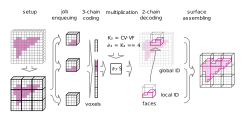
\includegraphics[width=\textwidth]{figs/schema_horizontal.pdf} 
%\includegraphics[scale=1]{input/ircad_comparison.pdf} 
\caption{Workflow of \textsc{lar-surf} algorithm}
\label{fig:schema}
\end{figure}

With $size=64$, the number of non-zeros within the sparse matrix $[\partial(64^3)]$ is $\mathtt{nnz} = 4 792 266$, for a memory size of $9\times \mathtt{nnz}+8\times 262144 \simeq 45$ MB. The memory size of the sparse matrix is computed by considering $8+1$ bytes for non-zero element (which are exactly 6 per row), plus 8 bytes per each index of column start.  


\subsubsection*{Job enqueuing}
% \subsubsection{Job enqueuing}
\label{sec:job-enq}
Communication and data synchronization may be managed through \emph{Channels}, which are the FIFO conduits that may provide producer/consumer communication. Overall execution time can be improved if other tasks can be run while a task is being executed, or while waiting for an external service/function to complete. The single work items of this stage follow:
\begin{enumerate}

\item extraction, from image arrays of the block views, depending on 3 Cartesian indices;

\item transform  each block \emph{from global} $[\ell_1]\times[\ell_2]\times[\ell_3]$ to \emph{local coordinates} $[n]\times[n]\times[n]$;

\item further transform of each \emph{foreground voxel} $\nu\in\mathcal{S}\subseteq\mathcal{I}$ from Cartesian to linear coordinates, using the suitable Julia's library functions.

\item enqueuing the job (as a sequence of integer positions for the non-zeros image elements aligned in a memory buffer of proper \texttt{Channel} type).
\end{enumerate}

\subsubsection*{3-Chain encoding}
\label{chain-coding}
The interesting part of the \emph{Image} $\mathcal{I}$ is called \emph{Segment} $\mathcal{S}$. The goal of the whole \emph{workflow} is to extract a \emph{boundary model} of $\mathcal{S}$ from $\mathcal{I}$. The portion of $\mathcal{S}$ inside $\mathcal{B}$, will be denoted as $\mathcal{S}(B)$.
Each block $\mathcal{B}$ of the 3D image must by converted into the \emph{coordinate representation} of a vector $\nu\in C_3$ in the linear space  of 3-chains. 

In coordinates local to $\mathcal{B}$, once fixed an ordering from Cartesian to linear coordinates, this vector is represented by a \emph{binary array} of length $size^3$. With $size=64$, we have $64^3=262144$,  with a non-zero value (i.e.~$1$) for each foreground voxel in $\mathcal{S}(B)$. Therefore, the coded segment portion $\mathcal{S}(B)$ results with a space occupancy of about $262$ KB if encoded as a full array (i.e.~including the zero values). Whether encoded as a sparse vector, its space occupancy will correspondingly decrease.

\begin{enumerate}

\item each encoding task produces either a full or sparse binary vector. With full or sparse arrays depending by one index, we get either 262 KB or less per job, correspondingly;

\item special format for sparse CSC (Compressed Sparse Column) vectors can be used, since the \emph{value} data for non-zeros does not need storage. Hence only a single 1-array of \texttt{Int64} row positions (with total length equal to the number of non-zeros in the block, with $8\times\mathtt{nnz}$ kB storage) is needed;

\item prepare subsequences of such data vectors (non-zero linear row indices), in order to feed efficiently the available processor threads.
In case of the presence of one/more GPUs, a smaller size of the block---and hence of the boundary matrix and the encoded 3-chain vectors---and then much higher vector numbers, are preferable for speed.

\end{enumerate}

\subsubsection*{SpMM Multiplication}\label{SpMM-multiplication}
According to the current literature~
\cite{Buluc2017} it is more convenient to execute SpMV (sparse matrix-vector) multiplications than SpMSpV (sparse matrix-sparse vector) multiplications. Since we have 256 such jobs (one multiplication per block) to perform in the default setting of the algorithm (
thize of the block $64^3$; the size of the image $512^2\times 256$), or more in case of either smaller blocks or image greater than the standard one, this stage must be evidently parallelized and carefully tuned, possibly by using the GPU, if available.
\begin{enumerate}

\item Various multiplication algorithms are being tested, using several packages for sparse linear algebra and/or custom implementations;

\item the total speed of this stage will strongly depend on the hardware available, on the granularity of blocks, and on the choice between dense/sparse storage of encoded 3-chains;

\item anyway, the compute elements or threads will be fed without solution of continuity in a \emph{dataflow} process. This parallel operation is, according to our preliminary experiments, the critical one of the whole workflow, in the sense that any $\Delta T$ (either positive or negative) in this stage will contribute to the total time $T$.

\end{enumerate}

\subsubsection*{2-Chain decoding}\label{sec:two-chain-decoding}
Each multiplication of $[\partial_B] : C_3 \to C_2$, times a 3-chain $\nu\in C_3$, produces a 2-chain  $\sigma\in C_2$, i.e.~the \emph{coordinate representation} of the \emph{boundary vector} $\sigma\in C_2$.  The inverse of the coding algorithm is executed in the present stage.  This process can also be partially superimposed in time with the previous ones, depending on the size of the memory buffers used to feed the CPU cores or the GPUs and get their results. Some elementary steps follow:

\begin{enumerate}

\item conversion from the position of ones (or non-zeros) in the 2-chain to linear indices of rows;

\item conversion from linear indices to Cartesian indices in coordinates local to the $\mathcal{B}$ block, using the appropriate library functions;

\item conversion from each Cartesian index value to a suitably oriented (i.e.~with proper attitude) geometry quadrilateral (or pair of triangles) in local coordinates.

\end{enumerate}

Julia's vectorized pipeline dataflow seems the more appropriate implementation model for the job of each worker.

\subsubsection*{Assembling and artifact filtering}\label{sec:artifact-filtering}
The results of the previous stages can be described as a \emph{collection of sets} of \emph{geometric quadrilaterals (quads)}, each one encoded as an array of quadruples of integer indices, pointing to the linear array of grid vertices associated to the image block $\mathcal{B}$.  In other words, \emph{all quads} of \textbf{each job} are now given in the \textbf{same} \emph{local coordinates}.  Besides putting each partial surface $\mathcal{S}(B) = (\texttt{V}_B, \texttt{FV}_\sigma)$ in the global coordinate system of the image, the present stage must eliminate the redundant boundary features possibly generated at the edges of the partial surface $\mathcal{S}(B)$ within each block $\mathcal{B}$ such that $B \cap \mathcal{I} \not= \emptyset$:

\begin{enumerate}

\item translate each array $\mathtt{FV}_\sigma$, of type \texttt{Lar.Cells}, by summing to each vertex index the linearized offset of the Cartesian coordinates $(n,m,p)(B)$ of the $\mathcal{B}$'s \emph{reference vertex}, i.e.~the one with (all) lowest \emph{Cartesian coordinates} within the $\mathcal{B}$ block.

\item remove both instances of \emph{double quads} generated by \texttt{Lar} software at the block boundaries 
(see Fig.~\ref{fig:brickboundary}). 
% TODO fix reference probably uncomment next line to link it to Figure 3
% (see Figure~\ref{fig:example}). 
They are artifacts generated by the decomposition of the whole image into a number of blocks of tractable size.

\item 
a smart strategy of removal of such artifacts may be used, which does not require any sorting nor searching on the assembled array of quads. It will consist in arranging each block with all three dimensions decreased-increased by one so that each 2-adjacent pair of blocks will be covering each other for a full side extent of blocks of depth one. 
% The details of this \emph{artifact filtering} are elucidated in  section~\ref{sec:covering}.
% TODO fix the reference
% TODO is there such a section?

\end{enumerate}

\subsubsection*{Smoothing}\label{sec:smoothing}
The final smoothing of the generated surfaces cannot be performed block-wise since this would introduce smoothing artifacts at the block boundaries. Anyway, the Taubin smoothing~\cite{Taubin1995} can be performed in parallel, since for each vertex in the final surface (except eventually the ones on the image $\mathcal{I}$ boundaries) it essentially consists in computing a new position as a proper average of its neighborhood vertices, i.e.~by applying a discrete Laplacian operator.  Some appropriate sets of workers may so be assigned the task of generating iteratively a new position for the vertices they take cure of. In particular, we have:
\begin{enumerate}

\item Job enqueuing, by writing sets of integers (global linear indices of vertices) in array buffers of type \texttt{Channel};

\item vectorized computation of proper averages of near vertices;

\item job dequeuing, by recovering finished tasks from a channel and assembling the results into the embedding function $\mathtt{V}: C_0 \to \E^3$, providing an array of type \texttt{Lar.Points} of \texttt{Float64 $\times$ 3}, with vertex coordinates by column.
\end{enumerate}



\subsection{Performance analysis}\label{sec:analysis}

\subsubsection*{Boundary matrix size}
The size of the boundary matrix is a critical parameter of the \textsc{lar-surf} method. To determine optimal size of boundary matrix the experiment on artificial data was performed (Fig.  \ref{fig:bm_size_tesla}). The size of experimental data is set to $512\times512\times512$ and it is derived from a typical size of Computed Tomography medical images. Computation is done on the Tesla DGX-1 machine.

According to the experiment the fastest computation is with the boundary matrix with size $64\times64\times64$. This is an expected result. The larger boundary matrix is too big to fit in CPU's cache memory.

\begin{figure}
\centering
\begin{subfigure}{0.495\textwidth}
\includegraphics[width=0.99\textwidth]{figs/bm_size_tesla.pdf} 
%\includegraphics[scale=1]{input/ircad_comparison.pdf} 
\subcaption{Time requirements of the \textsc{lar-surf} filter used on artificial volumetric data with various sizes of boundary matrix}
% \caption{Time requirements of LAR-SURF filter used on artificial with different size of boundary matrix}
\label{fig:bm_size_tesla}
\end{subfigure}
\begin{subfigure}{0.495\textwidth}

\includegraphics[width=0.99\textwidth]{figs/ircad_comparison.pdf} 
%\includegraphics[scale=1]{input/ircad_comparison.pdf} 
\subcaption{Time requirements of the LAR-SURF filter and Marching Cubes on the Ircad dataset. Error bars show the 95\% confidence interval}
\label{fig:ircad_comparison}
\end{subfigure}
\caption{Performance analysis of the \textsc{lar-surf} filter.}

\end{figure}


\subsubsection*{Comparison with the Marching Cubes algorithm}
To compare the time requirements of \textsc{lar-surf} with Marching Cubes implemented in Python we performed an experiment on Ircadb dataset \cite{ircadb}. Dataset contain 20 Computed Tomography images (see table \ref{tab:ircad2}) with xy-resolution from 0.56 mm to 0.87 mm and z-resolution from 1.0 mm to 4.0 mm. 
The number of slices is each series varies from 74 to 260 and the size of each slice is $512\times512$. 
The dataset contains manually segmented liver, portal vein, and other structures. We performed surface extraction of the liver with Marching Cubes and LAR-SURF. The time required for computation can be seen in Fig. \ref{fig:ircad_comparison}. 

Based on the t-test with $\alpha=0.99$, $p=\num[]{8.735e-24}$ and 
$s=\num[]{-16.67}$ it can be shown that the mean of time consumed by LAR-SURF is significantly lower from time consumed by Marching Cubes.


% \begin{figure}
% \centering
% \includegraphics[width=0.99\textwidth]{figs/ircad_comparison.pdf} 
% %\includegraphics[scale=1]{input/ircad_comparison.pdf} 
% \caption{Time requirements of LAR-SURF filter and Marching Cubes on Ircad dataset. Error bars shows the 95\% confidence interval}
% \label{fig:ircad_comparison}
% \end{figure}


\section{Examples}\label{sec:examples}


The 
For an experiments the we used the dataset Ircad1b. 

\begin{table}
\begin{tabular}{rrrrrr}
\toprule
 ID &  z-resolution [mm] &  xy-resolution [mm] &  obj. voxels &  size xy &  size z \\
\midrule
  1 &               1.60 &            0.570000 &      2865131 &      512 &     129 \\
  2 &               1.60 &            0.782000 &      1648024 &      512 &     172 \\
  3 &               1.25 &            0.625000 &      2375079 &      512 &     200 \\
  4 &               2.00 &            0.742188 &      1132427 &      512 &      91 \\
  5 &               1.60 &            0.782000 &      2124505 &      512 &     139 \\
  6 &               1.60 &            0.782000 &      1828493 &      512 &     135 \\
  7 &               1.60 &            0.782000 &      1461944 &      512 &     151 \\
  8 &               1.60 &            0.561000 &      3215090 &      512 &     124 \\
  9 &               2.00 &            0.873047 &      1265420 &      512 &     111 \\
 10 &               1.60 &            0.736000 &      1871804 &      512 &     122 \\
 11 &               1.60 &            0.720000 &      1692716 &      512 &     132 \\
 12 &               1.00 &            0.679688 &      3341433 &      512 &     260 \\
 13 &               1.60 &            0.671000 &      2063109 &      512 &     122 \\
 14 &               1.60 &            0.720000 &      1633641 &      512 &     113 \\
 15 &               1.60 &            0.782000 &      1389572 &      512 &     125 \\
 16 &               1.60 &            0.698000 &      2717185 &      512 &     155 \\
 17 &               1.60 &            0.743000 &      2106497 &      512 &     119 \\
 18 &               2.50 &            0.742188 &      1220564 &      512 &      74 \\
 19 &               4.00 &            0.703125 &       583208 &      512 &     124 \\
 20 &               2.00 &            0.808594 &      1359697 &      512 &     225 \\
\bottomrule
\end{tabular}

\end{table}
\begin{table}
\begin{tabular}{lrrrrr}
\toprule
{} &  z-resolution [mm] &  xy-resolution [mm] &   obj. voxels &  size xy &      size z \\
\midrule
count &           20.00000 &           20.000000 &  2.000000e+01 &     20.0 &   20.000000 \\
mean  &            1.77750 &            0.725141 &  1.894777e+06 &    512.0 &  141.150000 \\
std   &            0.60273 &            0.077233 &  7.206126e+05 &      0.0 &   44.088756 \\
min   &            1.00000 &            0.561000 &  5.832080e+05 &    512.0 &   74.000000 \\
25\%   &            1.60000 &            0.693422 &  1.382103e+06 &    512.0 &  121.250000 \\
50\%   &            1.60000 &            0.739094 &  1.760604e+06 &    512.0 &  127.000000 \\
75\%   &            1.70000 &            0.782000 &  2.187148e+06 &    512.0 &  152.000000 \\
max   &            4.00000 &            0.873047 &  3.341433e+06 &    512.0 &  260.000000 \\
\bottomrule
\end{tabular}

\end{table}

\section{Conclusion}\label{sec:conclusion}

% In this paper we have introduced and discussed a Julia implementation of an algebraic filter to extract from medical 3D images the boundary sourface of a specific image segment, described as a 3-chain of voxels. We have shown a good advantage over standard marchin-cubes algorithms. Translations from cartesian indices of cells to linearized indices, and the sparse matrix-vector multiplication are the main computational kernels of this approach. The current implementation employs Julia's channels for multiprocessing, and can be extended to gain a much greater speed-up using hybrid architectures mixing  CPUs and GPUs of last generation. 

% % TODO from abstract
% We introduced a Julia implementation of an algebraic filter to extract from 3D medical images the
% boundary surface of some specific image segment, described as a 3-chain of voxels. Translations from
% Cartesian indices of cells to linearized indices, the computation of the sparse boundary matrices, and the
% sparse matrix-vector multiplication are the main computational kernels of this approach. We may show
% a good speed-up over marching-cubes algorithms. The existing implementation employs Julia's channels
% for multiprocessing. Currently, the computational pipeline is being strongly improved to gain a greater
% speed-up using native Julia implementation \texttt{CUDA.jl} of Nvidia programming platform 
% % TODO cite Besard2017 [7]
% , and the Julia's
% \texttt{SuiteSparseGraphBLAS.jl} framework 
% % TODO cite BULUK 2017 [8] 
% for graph algorithms with the language of linear algebra. In
% particular, we are extending its use pattern in order to work with general cellular complexes.


We introduced a Julia implementation of an algebraic filter to extract from 3D medical images the
boundary surface of some specific image segment, described as a 3-chain of voxels. Translations from
Cartesian indices of cells to linearized indices, the computation of the sparse boundary matrices, and the
sparse matrix-vector multiplication are the main computational kernels of this approach. 

The implementation of the \textsc{lar-surf} filter is available in the open-source repository and it can be installed using standard Julia package manager \cite{larsurf-github}.

% NEW next two sentences are new
We showed a good speed-up over marching-cubes algorithms. 
The existing implementation employs Julia's channels
for multiprocessing. 
Our performance experiment showed an optimal size of the brick size.
Parallelization makes a large portion of spared computational cost. 
%
Moreover, we expect additional improvement in the future because our approach is appropriate  for SIMD (Single Instruction, Multiple Data) hybrid architectures of CPUs and GPUs, since only the initial block setup of boundary matrix and image slices, as well the final collection of computed surface portions, require inter-process communication. 

\sloppy{
Currently, the computational pipeline is being strongly improved to gain a greater
speed-up using native Julia implementation \texttt{CUDA.jl} of Nvidia programming platform 
% TODO cite Besard2017 [7]
% \cite{Besard:2017}
\cite{Besard2019}
, and Julia's
\texttt{SuiteSparseGraphBLAS.jl} framework 
\cite{Buluc2017}
% TODO cite BULUK 2017 [8] 
for graph algorithms with the language of linear algebra. In
particular, we are extending its use pattern in order to work with general cellular complexes.
}

\appendix
\section{Appendix}
\subsection{Symbol list}

\begin{description}
\item[$\mathcal{I}$]  three-dimensional medical image
\\[-8mm]
\item[$\ell_1, \ell_2, \ell_3$]  dimensions of image
\\[-8mm]
\item[$\mathcal{S}$]  segment: subset of voxels
\\[-8mm]
\item[$\mathcal{B}$] 3D image block 
\\[-8mm]
\item[$size$] lateral dimension of cubic block $\mathcal{B}$ 
\\[-8mm]
\item[$n$]	number of blocks $\mathcal{B}$ (jobs) in $\mathcal{I}$
\\[-8mm]
\item[[$\partial_\mathcal{B}$] ]  boundary matrix for block $\mathcal{B}$
\\[-8mm]
\item[$C_p$] linear (vector) space of $p$-chains
\\[-8mm]
\item[$\nu\in C_p$] $p$-chain
\\[-8mm]
\item[[$\nu$]] coordinate representation (binary vector) of  $\nu$
\\[-8mm]
\item[$\E^3$] Euclidean 3-space
\end{description}


\subsection{Definitions}
\begin{description}
\item[CSC]  Compressed Sparse Column format for sparse matrices
\\[-8mm]
\item[Global coordinates]  Integer linear coordinates of $\mathcal{I}$
\\[-8mm]
\item[Local coordinates] Integer linear coordinates of $\mathcal{B}$
\\[-8mm]
\item[Cartesian coordinates] Integer triples $(i,j,k)$ one-to-one with voxels 
\\[-8mm]
\item[Voxels] individual elements in 3D image (3-cells)
\\[-8mm]
\item[$p$-chain] formal linear combination of $p$-cells with coefficients in $\{0,1\}$
\\[-8mm]
\item[Coord. repr.]  binary vector (for $p$-chains) or binary matrix (for chain operators)
\\[-8mm]
\item[Quad]	geometric quadrilateral; convex polygon with four vertices 
\\[-8mm]
\item[Foreground voxel] individual element of a segment $\mathcal{S}$
\\[-8mm]
\item[Segment]	subset of voxels resulting from image segmentation
\end{description}


\bibliographystyle{alpha}
\bibliography{library}

\end{document}  
